%%%%%%%%%%%%%%%%%%%%%%%%%%%%%%%%%%%%%%%%%%%%%%%%%%%%%%%%%%%%%%%%%%%%%%%%%%%%%%%
% Chapter 'Adsorption - Water - silica gel pellet Fuji A'
%%%%%%%%%%%%%%%%%%%%%%%%%%%%%%%%%%%%%%%%%%%%%%%%%%%%%%%%%%%%%%%%%%%%%%%%%%%%%%%
\subsection{Silica gel pellet Fuji A}
%
%%%%%%%%%%%%%%%%%%%%%%%%%%%%%%%%%%%%%%%%%%%%%%%%%%%%%%%%%%%%%%%%%%%%%%%%%%%%%%%
%%%%%%%%%%%%%%%%%%%%%%%%%%%%%%%%%%%%%%%%%%%%%%%%%%%%%%%%%%%%%%%%%%%%%%%%%%%%%%%
\subsubsection{Freundlich - ID 1}
%
\begin{tabular}[l]{|lp{11.5cm}|}
\hline
\addlinespace

\textbf{Sorbent:} & silica gel pellet \\
\textbf{Subtype:} & Fuji A \\
\textbf{Refrigerant:} & Water \\
\textbf{Equation:} & Freundlich \\
\textbf{ID:} & 1 \\
\textbf{Reference:} & SAKODA, AKIYOSHI; SUZUKI, MOTOYUKI (1984): Fundamental study on solar powered adsorption cooling system. In: J. Chem. Eng. Japan / JCEJ 17 (1), S. 52–57. DOI: 10.1252/jcej.17.52. \\
\textbf{Comment:} & None \\

\addlinespace
\hline
\end{tabular}
\newline

\textbf{Properties of sorbent:}
\newline
%
\begin{longtable}[l]{lll}
\toprule
\addlinespace
\textbf{Property} & \textbf{Unit} & \textbf{Value} \\
\addlinespace
\midrule
\endhead
\bottomrule
\endfoot
\bottomrule
\endlastfoot
\addlinespace

Diameter of pellet & \si{\milli\meter} & 0.71\\

\addlinespace\end{longtable}

\textbf{Equation and parameters:}
\newline
%
Loading $w$ in $\si{\kilogram\per\kilogram}$ is calculated depending on pressure $p$ in $\si{\pascal}$, temperature $T$ in $\si{\kelvin}$, and vapor pressure $p_\mathrm{sat}$ in $\si{\pascal}$ by:
%
\begin{equation*}
\begin{split}
w &=& A \left( \nicefrac{p}{p_\mathrm{sat}} \right) ^{B} & \quad\text{, and} \\
A &=& A_0 + A_1 T + A_2 T^2 + A_3 T^3 & \quad\text{, and} \\
B &=& B_0 + B_1 T + B_2 T^2 + B_3 T^3 & \quad\text{.} \\
\end{split}
\end{equation*}
%
The parameters of the equation are:
%
\begin{longtable}[l]{lll|lll}
\toprule
\addlinespace
\textbf{Par.} & \textbf{Unit} & \textbf{Value} &	\textbf{Par.} & \textbf{Unit} & \textbf{Value} \\
\addlinespace
\midrule
\endhead

\bottomrule
\endfoot
\bottomrule
\endlastfoot
\addlinespace

$A_0$ & $\si{\kilogram\per\kilogram}$ & 3.460000000e-01 & $B_0$ & - & 6.250000000e-01 \\
$A_1$ & $\si{\kilogram\per\kilogram\per\kelvin}$ & 0.000000000e+00 & $B_1$ & $\si{\per\kelvin}$ & 0.000000000e+00 \\
$A_2$ & $\si{\kilogram\per\kilogram\per\square\kelvin}$ & 0.000000000e+00 & $B_2$ & $\si{\per\square\kelvin}$ & 0.000000000e+00 \\
$A_3$ & $\si{\kilogram\per\kilogram\per\cubic\kelvin}$ & 0.000000000e+00 & $B_3$ & $\si{\per\cubic\kelvin}$ & 0.000000000e+00 \\

\addlinespace\end{longtable}

\textbf{Validity:}
\newline
No data on validity available!
\newline

\textbf{Visualization:}
%
\begin{figure}[!htp]
{\noindent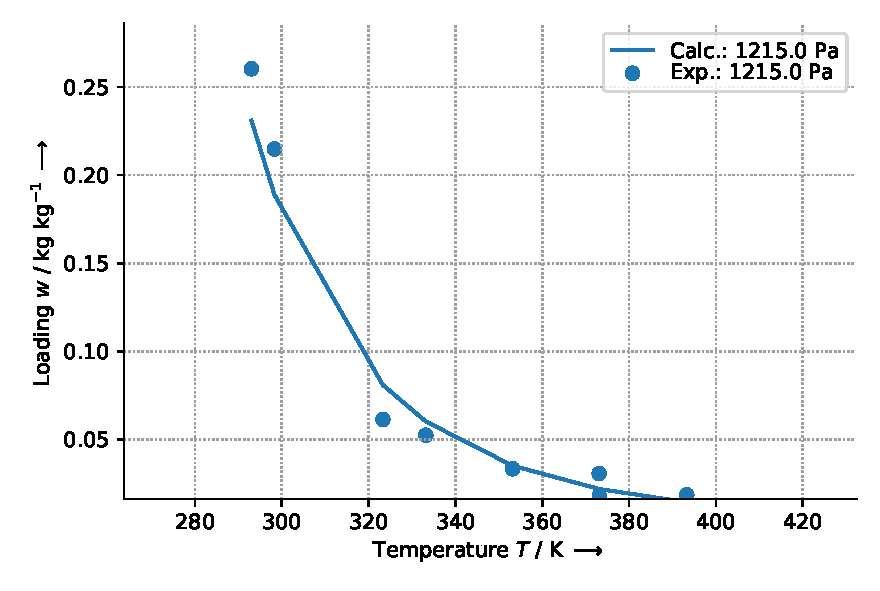
\includegraphics[height=10cm, keepaspectratio]{figs/ads/ads_Water_silica_gel_pellet_Fuji_A_Freundlich_1.pdf}}
\end{figure}
%

To generate the figure, the following refrigerant functions were selected:
\begin{itemize}
\item Vapor pressure: VaporPressure\_EoS1 - ID 1
\item Saturated liquid density: SaturatedLiquidDensity\_EoS1 - ID 1
\end{itemize}

The uncertainity of the experimental data is:
\begin{itemize}
\item Data source $\,\to\,$ Data was taken from figure
\end{itemize}

The mean absolute percentage error (MAPE) between the experimental and calculated data results in 18.64\%.
\FloatBarrier
\newpage
%%%%%%%%%%%%%%%%%%%%%%%%%%%%%%%%%%%%%%%%%%%%%%%%%%%%%%%%%%%%%%%%%%%%%%%%%%%%%%%
